%% BioMed_Central_Tex_Template_v1.06
%%                                      %
%  bmc_article.tex            ver: 1.06 %
%                                       %

%%IMPORTANT: do not delete the first line of this template
%%It must be present to enable the BMC Submission system to
%%recognise this template!!

%%% loading packages, author definitions

%\documentclass[twocolumn]{bmcart}% uncomment this for two column layout and comment line below
\documentclass{bmcart}

\usepackage{mathptmx}       % selects Times Roman as basic font
\usepackage{helvet}         % selects Helvetica as sans-serif font
\usepackage{courier}        % selects Courier as typewriter font
\usepackage{type1cm}        % activate if the above 3 fonts are not available on your system
\usepackage{makeidx}         % allows index generation
\usepackage{graphicx}        % standard LaTeX graphics tool when including figure files
\usepackage{multicol}        % used for the two-column index
\usepackage[bottom]{footmisc} % places footnotes at page bottom
\usepackage{subfig}
\usepackage{amsfonts}
\usepackage[cmex10]{amsmath}
\usepackage{float}
\usepackage[utf8]{inputenc}

\usepackage{bm} 
\usepackage{amsmath}
\usepackage{amssymb}

\usepackage{caption}

\usepackage{algpseudocode}
\usepackage{algorithm}

%%%%%%%%%%%%%%%%%%%%%%%%%%%%%%%%%%%%%%%%%%%%%%%%%
%%                                             %%
%%  If you wish to display your graphics for   %%
%%  your own use using includegraphic or       %%
%%  includegraphics, then comment out the      %%
%%  following two lines of code.               %%
%%  NB: These line *must* be included when     %%
%%  submitting to BMC.                         %%
%%  All figure files must be submitted as      %%
%%  separate graphics through the BMC          %%
%%  submission process, not included in the    %%
%%  submitted article.                         %%
%%                                             %%
%%%%%%%%%%%%%%%%%%%%%%%%%%%%%%%%%%%%%%%%%%%%%%%%%

%\def\includegraphic{}
%\def\includegraphics{}

%%% Put your definitions there:
\startlocaldefs
\endlocaldefs

%%% Begin ...
\begin{document}

%%% Start of article front matter
\begin{frontmatter}

\begin{fmbox}
\dochead{Research}

% Document information

\title{Estimation of flow trajectories in a multi-lines transportation network}

\author[
  addressref={aff1},                   
  corref={aff1},                       
  email={gguex@unil.ch}
]{\inits{G.G.}\fnm{Guillaume} \snm{Guex}}
\author[
  addressref={aff2},
  email={rloup@unil.ch}
]{\inits{R.L.}\fnm{Romain} \snm{Loup}}
\author[
addressref={aff1, aff2},
email={fbavaud@unil.ch}
]{\inits{F.B.}\fnm{François} \snm{Bavaud}}

\address[id=aff1]{%                           
  \orgdiv{Department of Language and Information Sciences},             
  \orgname{University of Lausanne},          
  \city{Lausanne},                              
  \cny{Switzerland}                                   
}
\address[id=aff2]{%
  \orgdiv{Institute of Geography and Sustainability},
  \orgname{University of Lausanne},          
  \city{Lausanne},                       
  \cny{Switzerland} 
}

\end{fmbox}

% The Abstract begins here                  

\begin{abstractbox}

\begin{abstract} % abstract
Characterizing a public transportation network, such as an urban multi-lines bus network, requires the origin-destination trip counts during a given period. Yet, if automatic counting makes the embarkment (boarding) and disembarkment (alighting) counts at each bus stop known, it often happens that pedestrian transfers between stops are unknown, and this contribution proposes a three-steps procedure for estimating the missing information, involving maximum entropy and iterative fitting. ** à poursuivre ***
\end{abstract}

% Keywords begin here  

\begin{keyword}
\kwd{multiline bus network}
\kwd{origin-destination flows}
\kwd{boarding and alighting counts}
\kwd{transit flows}
\kwd{maximum entropy estimation}
\end{keyword}

% MSC classifications codes, if any
%\begin{keyword}[class=AMS]
%\kwd[Primary ]{}
%\kwd{}
%\kwd[; secondary ]{}
%\end{keyword}

\end{abstractbox}

\end{frontmatter}

% Main Body

%% --------------------------------- INTRODUCTION

\section{Introduction}
% Alternative title: Estimating transit flows from boarding and alighting counts
Transportation networks determine our mobility, require a considerable amount of planning and resources, and elicit much public hopes and critics. 
They also constitute an endless source of inspiration in formal modeling and optimization, as attested in operations research (classical optimal transportation, maximum flow problem), quantitative geography and spatial econometrics (spatial navigation, multimodality, gravity models for flows), and machine learning (recent developments in regularized optimal transportation, such as color transfer or images interpolation; see e.g. \cite{peyre2019computational}). 

This contribution adresses a straightforward, yet central question  in public transportation networks: given a network made of many bus lines, how can one estimate the real trips made by the travelers, on the sole basis of  the embarkment (boarding) counts and disembarkment (alighting) counts for each bus stop? Although estimating origin-destination flows is a much addressed issue in transportation modeling (see e.g \cite{bell1997transportation} \cite{hazelton2000estimation} \cite{ashok2002estimation} \cite{cui2006bus} and references therein), the specific problem addressed in this contribution seems, to the best of our knowledge, original. 


Pedestrian transfers of travelers between bus lines here constitute the missing information, whose principled evaluation require some methodological reflexion and experimentation. Section \ref{notforma} introduces the notations and the formalism, as well as the statement of the problem and the iterative solution method, which consist of three consecutive steps: a maximum-entropy computation of the trip distributions, obeying marginal constraints and with a given prior (section \ref{maxenso}); an update of the marginal flows to avoid transfer overflow (section \ref{marginup}); and an update of the prior distribution  (section \ref{priorup}) by shrinking the components responsible for overflow. 

The fist step only is required for solving the single line case (section \ref{Single line}), naturally much simpler but  yet  not trivial, and exhibiting a disembarking probability independent of the embarking stop (Markov property). 

Cases studies are presented in section \ref{casestudies} *** à poursuivre *** 





%% --------------------------------- NOTATIONS AND FORMALISM

\section{Notations and formalism}
\label{notforma}
\subsection{Lines, stops  and junctions}
\label{Lines and junctions}
Consider a transportation network made of bus lines numbered $\ell=1,\ldots, q$, of respective lengths (number of stops) $l_\ell$.  Opposite lines, that is parallel lines running in the back and forth directions are considered as distinct. 

The $l=\sum_{\ell=1}^ql_\ell$ bus stops constitute the nodes of the transportation network. Each stop $i=1,\ldots,l$ belongs to {\em  a single bus line}, and defines a unique next or forward stop $F(i)$ (unless $i$ is the line terminus) and a unique backward stop $B(i)$ (unless $i$ is the line start), both on the same line.  

Let $S_i$ denote the set of stops which can be reached from stop $i$ within walking distance, excluding $i$ itself. A stop $i$ is referred to as an {\em isolated stop} if $S_i=\emptyset$, and to as a {\em junction} otherwise. 


\subsection{Line edges, transfer edges and trips}
\label{Line edges, transfer edges and trips}
Two sorts of oriented edges are involved in the transportation network: 
\begin{enumerate}
  \item[$\bullet$] intra-line edges $(i,j)=(i,F(i))$ belonging to a single line  $\ell(i)=\ell(j)$
  \item[$\bullet$] inter-line or transfer edges $(i,j)$ connecting different lines $\ell(i)\neq \ell(j)$, involving walks from junction $i$ to $j\in S_i$.
  \end{enumerate}
A $st$-trip, noted $[s,t]$, consists of entering into the network at stop $s$, and leaving the network at $t$, by following the shortest-path (i.e. achieving the minimum distance,  minimum time, or  minimum cost), supposed unique, leading to $s$ from $t$. 

The succession of edges $(ij)$ belonging to the $st$-trip, noted $(ij)\in [s,t]$, is unique. Define the edge-trip incidence matrix as
\begin{equation}
\label{edgetrip}
\chi_{ij}^{st} = \begin{cases}
  1    & \text{if $(ij)\in [s,t]$}, \\
  0    & \text{otherwise}.
\end{cases}
\end{equation}
A $st$-trip always starts with the edge $(s,F(s))$, and finishes with $(B(t),t)$. Transfers can occur in-between, but never at the beginning nor at the end of the trip. 

\vspace*{0.1cm}

\subsection{Transportation flows}
\label{Transportation flows}
Let  $x_{ij}$ count the number of travelers using edge $(ij)$ in a given period, such as a given hour, day, week or  year.  The edge flow $x_{ij}$ is denoted by $y_{ij}$ for an intra-line edge $(i,j)$, and 
by $z_{ij}$ for a transfer edge $(i,j)$. By construction, $x_{ij}=y_{ij}+z_{ij}$, where $y_{ij}\,  z_{ij}=0$. 

\vspace*{0.1cm}


Let $a_i$, respectively $b_i$, the number of passengers embarking, respectively disembarking at stop $i$. By construction, 
\begin{equation}
\label{bilan1ligne}
\begin{cases}
 y_{i,F(i)}=a_i \text{\,  and } b_i=0   & \text{if $i$ is a line start}, \\
y_{B(i),i}=b_i \text{\,  and } a_i=0   & \text{if $i$ is a line terminus}, \\
 y_{i,F(i)}=y_{B(i),i}+a_i-b_i     & \text{otherwise}.
\end{cases}
\end{equation}
Also, $\mathbf{a}$ and $\mathbf{b}$ must be consistent, in the sense that $A_i\ge B_i$, where $A_i$ (respectively $B_i$) is the cumulated number of embarked 
(resp. disembarked) passengers on the line under consideration, recursively defined as $A_{F(i)}=A_i+a_i$ (resp. $B_{F(i)}=B_i+b_i$). Moreover,  $A_i=B_i$ at a terminal line stop $i$. This common value yields  the total number of passengers transported by the line. 



\vspace*{0.1cm}

Let the transportation flow $n_{st}$ denote the number of passengers following an $st$-trip, that is entering the network at $s$ and leaving the network at $t$ by using the shortest path. One gets from (\ref{edgetrip}) 
\begin{equation}
\label{equationGG}
x_{ij}=\sum_{st}\chi_{ij}^{st}\:  n_{st}
\end{equation}
Among the passengers embarking in $i$, some transfer from another line, and some others enter into the network: 
\begin{equation}
\label{entrer}
a_i=z_{\bullet i}+n_{i\bullet}
\end{equation}
where  ``$\bullet$" denotes the summation over the replaced index, as in $n_{i\bullet}=\sum_{j=1}^l n_{ij}$. Similarly, among the passengers disembarking in $i$, some transfer to another line, and some others leave the network: 
\begin{equation}
\label{sortir}
b_i=z_{i\bullet}+n_{\bullet i}
\end{equation}
By construction
\begin{displaymath}
a_{\bullet}=b_{\bullet}=z_{\bullet\bullet}+n_{\bullet\bullet}
\end{displaymath}
where $n_{\bullet\bullet}$ counts the number of passengers, and $z_{\bullet\bullet}$ counts the number of transfers. $z_{\bullet\bullet}/n_{\bullet\bullet}$  is the average number of transfers per passenger. 

\vspace*{0.1cm}



As explained in section \ref{Lines and junctions}, transfers can only occur at junctions, that is $z_{ij}>0$ implies $j\in S_i$. In particular,  $z_{ii}=0$ : no traveller is supposed to disembark and re-embark later at the same stop. 


 
\subsection{Statement of the problem and solution method}
Automatic passenger counters measure the number of passengers entering and leaving buses at each stop [Boyle, 1998], that is $\mathbf{a}$ and $\mathbf{b}$, which provide the basic raw data of the present study, kindly provided by the Lausanne Transportation Agency (tl), after some preliminary, undocumented corrections (i.e. the components of $\mathbf{a}$ and $\mathbf{b}$ can be non-integer). It may also happen that, on some lines $\ell$,  raw data do not obey the necessary consistency condition  $a_\bullet^\ell=b_\bullet^\ell$ (where the latter quantities denote the total embarkments and disembarkments on line $\ell$), in which case we did rescale the embarking and disembarking line counts as 
\begin{displaymath}
\hat{a}_i=(1-\frac{a_\bullet^\ell-b_\bullet^\ell}{a_\bullet^\ell+b_\bullet^\ell})\, a_i 
 \qquad\qquad\qquad
  \hat{b}_i=(1+\frac{a_\bullet^\ell-b_\bullet^\ell}{a_\bullet^\ell+b_\bullet^\ell})\,  b_i 
\end{displaymath}
ensuring $\hat{a}_\bullet^\ell=\hat{b}_\bullet^\ell=2a_\bullet^\ell b_\bullet^\ell/(a_\bullet^\ell+b_\bullet^\ell)$. However, strongly unbalanced lines such that  $|a_\bullet^\ell-b_\bullet|^\ell/a_\bullet^\ell > 0.3$ or $|a_\bullet^\ell-b_\bullet^\ell|/b_\bullet^\ell > 0.3$  (which always turned out to be temporary lines with small  counts) were simply disregarded and line $\ell$ removed from the network. 

Also, the geometry of the network permits to derive the edge-trip incidence matrix $\bm{\chi}$ defined in (\ref{edgetrip}). 


Intra-line edge flows $\mathbf{Y}=(y_{ij})$ can be determined by (\ref{bilan1ligne}), but transfer edge flows $\mathbf{Z}=(z_{ij})$ are, here and typically, unknown. The objective is to estimate the $l\times l$ transportation flow $\mathbf{N}=(n_{st})$. Many consistent solutions coexist in general, even for a single line with no transferts (section \ref{Single line}). This issue of incompletely observed data can be tackled by the maximum entropy formalism \cite{jaynes1957information}, and has been often  in transportation modelling \cite{wilson1967statistical}  \cite{erlander1990gravity}. 



Let $f_{st}=n_{st}/n_{\bullet\bullet}$ be the proportion of $st$-trips (empirical distribution) and let $g_{st}$ be some prior guess on its shape (theoretical distribution). 
Assuming some reasonable initial prior $g_{st}$, 
\begin{itemize}
\item[(1)] we shall first suppose that the empirical margins $\alpha_s=f_{s\bullet}$ and $\beta_t=f_{\bullet t}$ are known.  
Then $f_{st}$ can be determined as the maximum entropy solution (section \ref{maxenso}), i.e. as the distribution closest to $g_{st}$ in the Kullback-Leibler divergence sense under the margin constraints, to be calibrated by an iterative fitting inner loop
\item[(2)] then (section \ref{marginup}), the margins will be updated to $\tilde{\alpha}_s$ and $\tilde{\beta}_t$   by requiring a minimum proportion $\theta\in (0,1)$ of passengers entering/leaving the network at each stop, as well as avoiding transfer overflow exceeding the embarking and disembarking counts at each stop
 \item[(3)] finally (section \ref{priorup}), the prior will be updated to $\tilde{g}_{st}$ by shrinking, if necessary, the priors $g_{st}$ associated to overflows. 
\end{itemize}
With the new prior distribution $\widetilde{g}_{st}$ and the new margin distributions $\widetilde{\alpha}_s$, $\widetilde{\beta}_t$, we can iterate the 
 the above steps, until convergence. The only free parameter is $\theta$, which will be discussed in section *** . 
 
 
 *** The above iterative solution method is somewhat reminiscent of the EM algorithm. As a matter of fact, the first  step  (maximum entropy) exactly correspond to the ``expectation step" of the EM algorithm (see e.g. \cite{dempster1977maximum}  \cite{bavaud2009information}), but steps two and three, aiming at calibrating the parameters $\bm{\alpha}$, $\bm{\beta}$ and $\mathbf{g}$, do not follow the maximum likelihood rationale of the ``maximisation step". 
 






\subsubsection{Maximum entropy estimate of $st$-trips}
\label{maxenso}
As announced,  the proportion of $st$-trips $f_{st}=n_{st}/n_{\bullet\bullet}$ (empirical distribution) will be estimated from some prior guess $g_{st}$ (theoretical distribution) and 
margin constraints $\alpha_s$ and $\beta_t$ for $f_{st}$ by maximum entropy, i.e. by 
solving the problem 
\begin{align}
	\label{constr_MaxEnt}
	\min_{\mathbf{f}\in\mathcal{F}} &\; \sum_{st}f_{st}\log \frac{f_{st}}{g_{st}}, \notag \\
	s.t. &\; \sum_t f_{st} = \alpha_s, \notag \\
	&\; \sum_s f_{st} = \beta_t.
\end{align}
The Lagragian is
\begin{equation}
	L = \sum_{st}f_{st}\log \frac{f_{st}}{g_{st}} - \sum_s \lambda_s (\alpha_s - \sum_t f_{st}) - \sum_t \mu_t (\beta_t - \sum_s f_{st}), \notag
\end{equation}
which gives, after deriving and setting to zero,
\begin{equation}
	\label{Sol}
	f_{st} = \phi_s \psi_t g_{st} \qquad \text{with } \phi_s := \exp(- 1 - \lambda_s) \text{, } \psi_t := \exp(- \mu_t).
\end{equation}
Using constraints in (\ref{constr_MaxEnt}), we find
\begin{equation}
	\label{Sol_LagMult}
	\phi_s = \frac{\alpha_s}{\sum_t \psi_t g_{st}}, \qquad \psi_t = \frac{\beta_t}{\sum_s \phi_s g_{st}}, 
\end{equation}
which yields the following \emph{iterative fitting algorithm}: starting with some $\psi^{(0)}_t > 0$, one performs the iteration
\begin{equation}
	\label{Iterative fitting}
	\phi^{(\iota)}_s = \frac{\alpha_s}{\sum_t \psi^{(\iota)}_t g_{st}}, \qquad \psi^{(\iota + 1)}_t = \frac{\beta_t}{\sum_s \phi^{(\iota)}_s g_{st}}, 
\end{equation}
until convergence to $\phi_s$ and $\psi_t$ obeying (\ref{Sol_LagMult}). 

In view of (\ref{entrer}) and (\ref{sortir}), the postulated margins must satisfy, for each isolated stop $i$
\begin{equation}
\label{ }
\alpha_i=\frac{a_i}{n_{\bullet \bullet}}\qquad\qquad \beta_i=\frac{b_i}{n_{\bullet \bullet}}
\end{equation}
permitting to determine the total flow as $n_{\bullet \bullet}=\frac{a_i}{\alpha_i}$, or  $n_{\bullet \bullet}=\frac{b_i}{\beta_i}$ for any isolated stop $i$, and thus 
the $st$-flow itself as 
\begin{equation}
	\label{flow_from_distrib}
	n_{st} = n_{\bullet \bullet} f_{st}= n_{\bullet \bullet}\phi_s \psi_t g_{st} 
\end{equation}
whose plugging into (\ref{equationGG}) yields the intra-line edge flows $\mathbf{Y}=(y_{ij})$ and the transfer edge flows $\mathbf{Z}=(z_{ij})$.


\subsubsection{Initialization of the prior and the margins}
The geometry of the network permits to rule out forbidden $st$-paths, i.e. obeying  $\chi^{st}_{\bullet\bullet}=0$. Such forbidden $st$-paths consist of *** @G? donner une liste exhaustive de critères d'exclusion ici ? ***  The initial prior was chosen as the uniform distribution on the remaining $c<l^2$ admissible $st$-paths, *** @G: que vaut $l$? que vaut $c$? ***,  that is as
\begin{equation*}
g_{ij} = \begin{cases}
  \frac{1}{c}    & \text{if $\chi^{st}_{\bullet\bullet}>0$}, \\
  0    & \text{otherwise}.
\end{cases}
\end{equation*}
The initial margins were chosen as  those of the flow without transfer, namely $\alpha_i=\frac{a_i}{a_{\bullet}}$ and $\beta_i=\frac{b_i}{b_\bullet}$ for all stops. 



\subsubsection{Updating  the margin distributions}
\label{marginup}
Let us define the hyperparameter $ \theta\in [0, 1)$ as the \emph{minimum proportion of passengers (among $a_i$ and $b_i$) entering/leaving the network at each stop}, that is $n_{s\bullet}\ge \theta a_s$ and $n_{\bullet t}\ge \theta b_t$. Note that we could set a different hyperparameter for each node, and differing for embarkments and disembarkments, but without addition information, we will restrain to this simpler case. Identities (\ref{entrer}) and  (\ref{sortir}) then imply the inequalities
\begin{displaymath}
z_{\bullet s} \le (1 - \theta) a_s\qquad\qquad \qquad z_{t \bullet} \le  (1 - \theta) b_t
\end{displaymath}
the violation of which constitutes transfer overflow. Hence requiring a minimal transfer yet avoiding overflow can be granted with the following updating of margins
\begin{equation}
\label{alpha_beta_update}
\widetilde{\alpha}_s = \frac{\min(\theta a_s, a_s - z_{\bullet s})}{\sum_{s'} \min(\theta a_{s'}, a_{s'} - z_{\bullet {s'}})}   \qquad \qquad \qquad
	\widetilde{\beta}_t = \frac{\min(\theta b_t, b_t - z_{t \bullet})}{\sum_{t'} \min(\theta b_{t'}, b_{t'} - z_{{t'} \bullet})}  \enspace. 
\end{equation}
 

\subsubsection{Updating the prior distribution}
\label{priorup}
Overflow occurs in transfer edge $(i, j)$ if  $z_{i \bullet} > (1 - \theta)b_i$ or $z_{\bullet j} > (1 - \theta)a_j$. To avoid it, components $g_{st}$ of the prior distribution 
will be shrinked by a suitable ratio whenever edge flows $(i,j)\in [s,t]$ exhibit overflow. 


 For any edge $(i, j)$, let us compute the \emph{flow ratio} $r_{ij}$ as
\begin{equation}
	\label{flow_ratio}
	r_{ij} = \max \left(1, \frac{z_{i \bullet}}{(1 - \theta)b_i}, \frac{z_{\bullet j}}{(1 - \theta)a_j} \right)\: \ge\: 1\enspace,
\end{equation}
where $r_{ij} > 1$ denotes an overflow through edge $(i, j)$. For a given origin-destination $[s,t]$, define the \emph{orgin-destination flow ratio} $\bar{r}_{st}$ 
as the largest $r_{ij}$ among edge flows $(i,j)\in [s,t]$, that is as 
\begin{equation}
	\label{st_flow_ratio}
	\bar{r}_{st} = \max_{ij} \chi_{ij}^{st} r_{ij}\: \ge\: 1\enspace.
\end{equation}
By construction, $\bar{r}_{st} > 1$ denotes an overflow on some transfer edge between $s$ and $t$. To adjust the flow, we shall divide the previous flow by this ratio
\begin{equation}
	\label{update_flow}
	\widetilde{n}_{st} =\frac{n_{st}}{\bar{r}_{st}}
\end{equation}
and define the new prior distribution  as
\begin{equation}
	\label{update_distrib}
	\widetilde{g}_{st} = \frac{\left( \frac{\widetilde{n}_{st}}{\phi_s \psi_t} \right)}{\sum_{s',t'} \left( \frac{\widetilde{n}_{s',t'}}{\phi_{s'} \psi_{t'}} \right)}\enspace. 
\end{equation}
where $\phi_s$ and $\psi_t$ are the values (\ref{Sol_LagMult}) obtained in the previous maximum entropy step. 

\subsubsection{Algorithm pseudocode}

\begin{algorithm}[H]
	\caption{Compute the transportation flow matrix $\mathbf{N} = (n_{st})$ knowing the edge-trip incidence matrix $\bm{\chi} = (\chi_{ij}^{st})$, the set of transfer edges $\mathcal{T}$, the embarking flow $\mathbf{a}$, the disambarking flow $\mathbf{b}$, the index of an isolated source node $\tilde{s}$, and the minimum proportion of passengers entering/leaving the network $\theta$.}
	\label{algo1}
	\begin{algorithmic}[1]
		\State $g_{st} \leftarrow I(\chi_{\bullet \bullet}^{st} > 0) / \sum_{s't'}I(\chi_{\bullet \bullet}^{s't'} > 0), \; \forall s,t$ \Comment{{\footnotesize Initialize the prior distribution}}
		
		\State $\alpha_s \leftarrow a_s / a_\bullet, \; \forall s$ \Comment{{\footnotesize Initialize the network ingoing distribution}}
		
		\State $\beta_t \leftarrow b_t / b_\bullet, \; \forall t$ \Comment{{\footnotesize Initialize the network outgoing distribution}}
		
		\State $\epsilon \leftarrow 10^{-40}$ \Comment{{\footnotesize Fix a small quantity}}
		
		\While{$\mathbf{N} = (n_{st})$ has not converge} \Comment{{\footnotesize Main loop}}
		
		\State $\psi_t \leftarrow 1, \; \forall t$
		
		\While{$\bm{\psi} = (\psi_t)$ has not converge} \Comment{{\footnotesize Iterative fitting loop}}
		
		\State $\phi_s \leftarrow \alpha_s / (\sum_t \psi_t g_{st} + \epsilon), \; \forall s$
		\State $\psi_t \leftarrow \beta_t / (\sum_s \phi_s g_{st} + \epsilon), \; \forall t$
		
		\EndWhile
		
		\State $n_{st} \leftarrow \frac{a_{\tilde{s}}}{\alpha_{\tilde{s}}} \phi_s \psi_t g_{st}, \; \forall s,t$ \Comment{{\footnotesize Compute the transportation flow}}
		
		\State $z_{ij} \leftarrow I((i,j) \in \mathcal{T})\sum_{st} \chi_{ij}^{st} n_{st}, \; \forall i,j$
		
		\State $\alpha_s \leftarrow \frac{\min(\theta a_s, a_s - z_{\bullet s})}{\sum_{s'} \min(\theta a_{s'}, a_{s'} - z_{\bullet {s'}})}, \; \forall s$ \Comment{{\footnotesize Update the network ingoing distribution}}
		
		\State $\beta_t \leftarrow \frac{\min(\theta b_t, b_t - z_{t \bullet})}{\sum_{t'} \min(\theta b_{t'}, b_{t'} - z_{{t'} \bullet})}, \; \forall t$ \Comment{{\footnotesize Update the network outgoing distribution}}
		
		\State $r_{ij} \leftarrow \max \left(1, \frac{z_{i \bullet}}{(1 - \theta)b_i}, \frac{z_{\bullet j}}{(1 - \theta)a_j} \right), \; \forall i,j$
		
		\State $\bar{r}_{st} \leftarrow \max_{ij} \chi_{ij}^{st} r_{ij}, \; \forall s,t$
		
		\State $\widetilde{g}_{st} \leftarrow \frac{\left( \frac{n_{st}}{\phi_s \psi_t \bar{r}_{st} + \epsilon} \right)}{\sum_{s',t'} \left( \frac{n_{s't'}}{\phi_{s'} \psi_{t'}\bar{r}_{s't'} + \epsilon} \right) + \epsilon}, \; \forall s,t$ \Comment{{\footnotesize Update the prior distribution}}
		
		\EndWhile
		\State \Return $\mathbf{N} = (n_{st})$
	\end{algorithmic}
\end{algorithm}


\subsection{Markov property for a single line}
\label{Single line}
A ``network" made of a single line contains no transfers, and flow estimates can be obtained at once by the maximum entropy step only.


Let  $i=1,\ldots, l$ enumerate the bus stops in increasing order,  i.e. $F(i)=i+1$. The initial prior is simply $g_{st}=c\; I(s<t)$ and captures solely the unidirectional nature of trips,  where $I(.)$ denotes the 0/1  indicator function and $c=\frac{1}{(l-1)(l-2)}$.   The margins of the empirical distribution $f_{st}$, as well as the total flow, are here known : 
\begin{displaymath}
\alpha_s=\frac{a_s}{a_\bullet}\qquad\qquad\qquad \beta_t=\frac{b_t}{b_\bullet}\qquad\qquad\qquad n_{\bullet\bullet}=a_{\bullet}=b_\bullet\enspace. 
\end{displaymath}
Following  (\ref{Sol}) maximum entropy flows are of the form
\begin{equation}
\label{nosignle}
n_{st}= n_{\bullet\bullet}\,  c\, I(s<t)\, \phi_s\,  \psi_t 
\end{equation}
where (setting $\Psi_s:=\sum_{t>s}\psi_t$ and $\Phi_t:=\sum_{s<t}c\phi_s$) the constraints (\ref{Sol_LagMult}) equivalently read
\begin{equation}
\label{dis embarking constraints}
\phi_s=\frac{\alpha_s}{c\, \sum_{t>s}\psi_t}=\frac{a_s}{n_{\bullet\bullet}\,  c\, \Psi_s}
\qquad\qquad\qquad
\psi_t=\frac{\beta_t}{c\, \sum_{s<t}\phi_s}=\frac{b_t}{n_{\bullet\bullet}\, c\, \Phi_t}
\end{equation}
to be solved by iterative fitting. 

Interestingly enough, the form (\ref{nosignle}) for the flows is reminiscent of the {\em gravity flows} of quantitative Geography \cite{wilson1967statistical}  \cite{erlander1990gravity} \cite{bavaud2002quasi} \cite{Thomas-Agnan2021}, where 
$\phi_s$ is the {\em push factor}, $\psi_t$ is the {\em pull factor}, and $I(s<t)$ the {\em distance deterrence function}. Yet, instead of  
being symmetric in $s,t$ and decreasing with the distance $|s-t|$, the distance deterrence function is here asymmetric due to the line orientation, but otherwise constant. 

This constancy entails the following Markovian behaviour for flows: let $m_{st}$ be the number of travelers embarking at stop $s$ and still inside the bus at stop $t>s$, and let $\rho_{st}$ the probability that travelers embarking at $s$ will disembark at $t$. By (\ref{nosignle}), 
\begin{displaymath}
m_{st}=\sum_{u\ge t}n_{su}=n_{\bullet\bullet}\, c\, \phi_s  \sum_{u\ge t} I(s<u)\, \psi_u =n_{\bullet\bullet}\, c\,  \phi_s (\psi_t+\Psi_t) 
\end{displaymath}
The empirical estimate of $\rho_{st}$ is given by the proportion, among the travelers embarking at $s$ and 
 still present at $t>s$,  of travelers disembarking at $t$, that is 
\begin{displaymath}
\rho_{st}=\frac{n_{st}}{m_{st}}=\frac{n_{\bullet\bullet}\, c\,  \phi_s\,   \psi_t}{n_{\bullet\bullet}\, c\,  \phi_s (\psi_t+\Psi_t)}=\frac{\psi_t}{\psi_t+\Psi_t}\le 1 
\end{displaymath}
which depends on $t$ only: it appears that the disembarkment probability $\rho_t=\frac{\psi_t}{\psi_t+\Psi_t}$ at $t$ is {\em independent} of the embarkment stop $s$. Said otherwise, a traveler embarking at any stop $s$ (and thus necessarily in the bus at $F(s)=s+1$) experiences the {\em same disembarkment probability} at each further stop $t>s$. 


This Markov property, enjoyed by maximum-entropic flows, contrasts other possible solutions, such as  the ``first in, first out" (FIFO) flows (homogenizing the 
traveled distances among users) or the ``last in, first out" (LIFO) flows (tending to generate maximally  contrasted traveled distances).


***  @G, ici davantage de développements sur l'approche Markovienne, ainsi que le joli schéma ?  ***


\

*** @G, @R, ici la (les) figure de l'exemple  ``starting from Maladière, Riant-Cour, Dapples"... ? ***

 
%% --------------------------------- CASE STUDIES

\section{Case Studies}
\label{casestudies}

Case studies are divided in two sections. In the first section, we test the algorithm on toy examples, which are artifical networks where the transportation flow $n_{st}$ is randomly drawn. These examples enable some kind of validation of the algorithm, as "real" transportation flows are known and can be compared to the solutions given by our method. This setup differs from the second section, which is dedicated to applying the algorithm to the real case of the public transportation network of the city of Lausanne (tl), where embarkement and disembarkement flows are measured but transportation flows are unknown. This second case study shows that the algorithm is applicable on large, real datasets and can gives insights about passengers probable routes in the network.

\subsection{Toy Examples}

\subsubsection{Examples construction}
\label{example_construction}

All constructed toy examples are built following the same approach, which aims at being simple but somewhat realistic. We fix a number of \emph{line tours} $p \geq 2$, each of which is constituted of a forward line and a backward line, for a total of $q = 2p$ lines. Every line has a starting and ending node, which are isolated node, and posses $p-1$ intermediary nodes which allows transfers to the other tour lines, giving a total of $n = 2p(p + 1)$ nodes in the network. Examples of these toy networks can be found in Figure \ref{toy_example_plots}.

\begin{figure}
	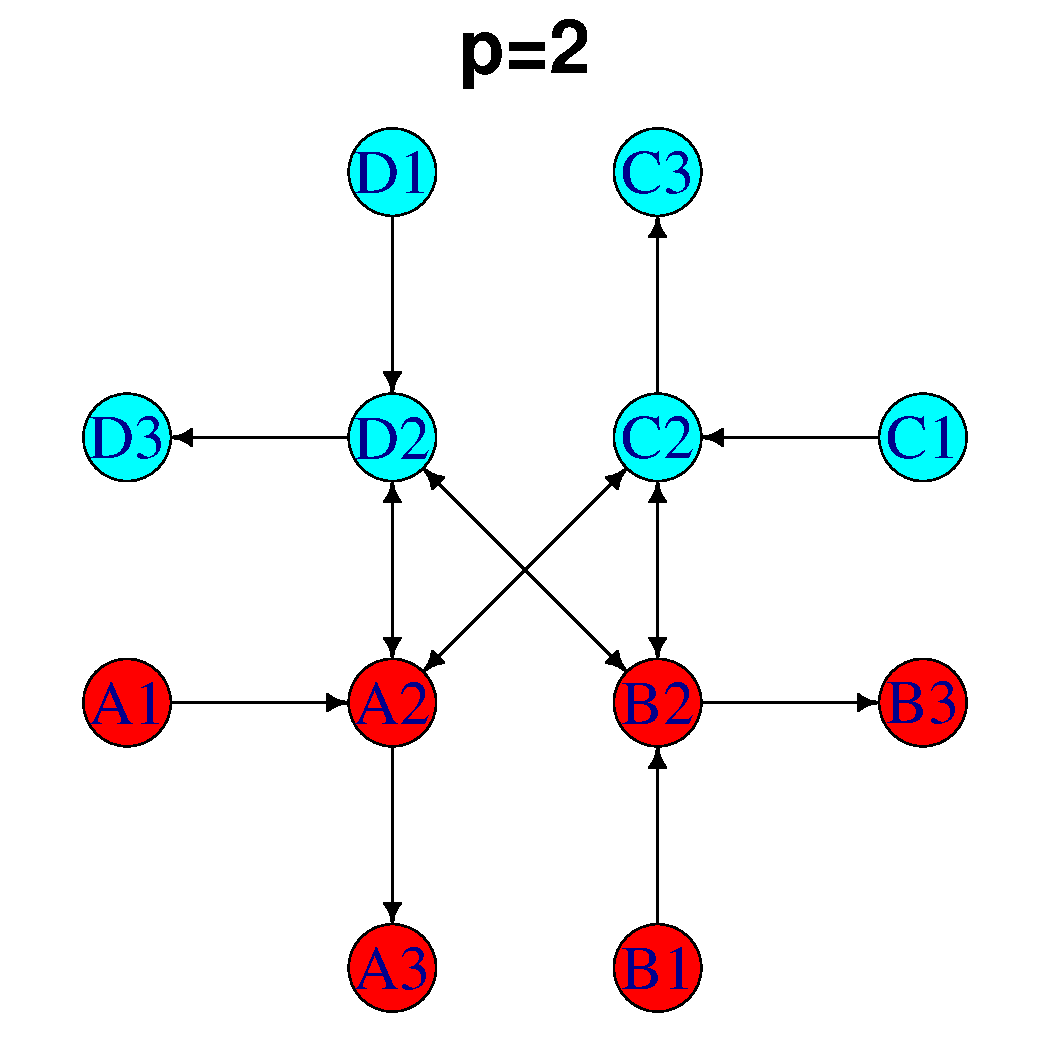
\includegraphics[width=0.3\textwidth]{fig/toy_2_display.pdf}
	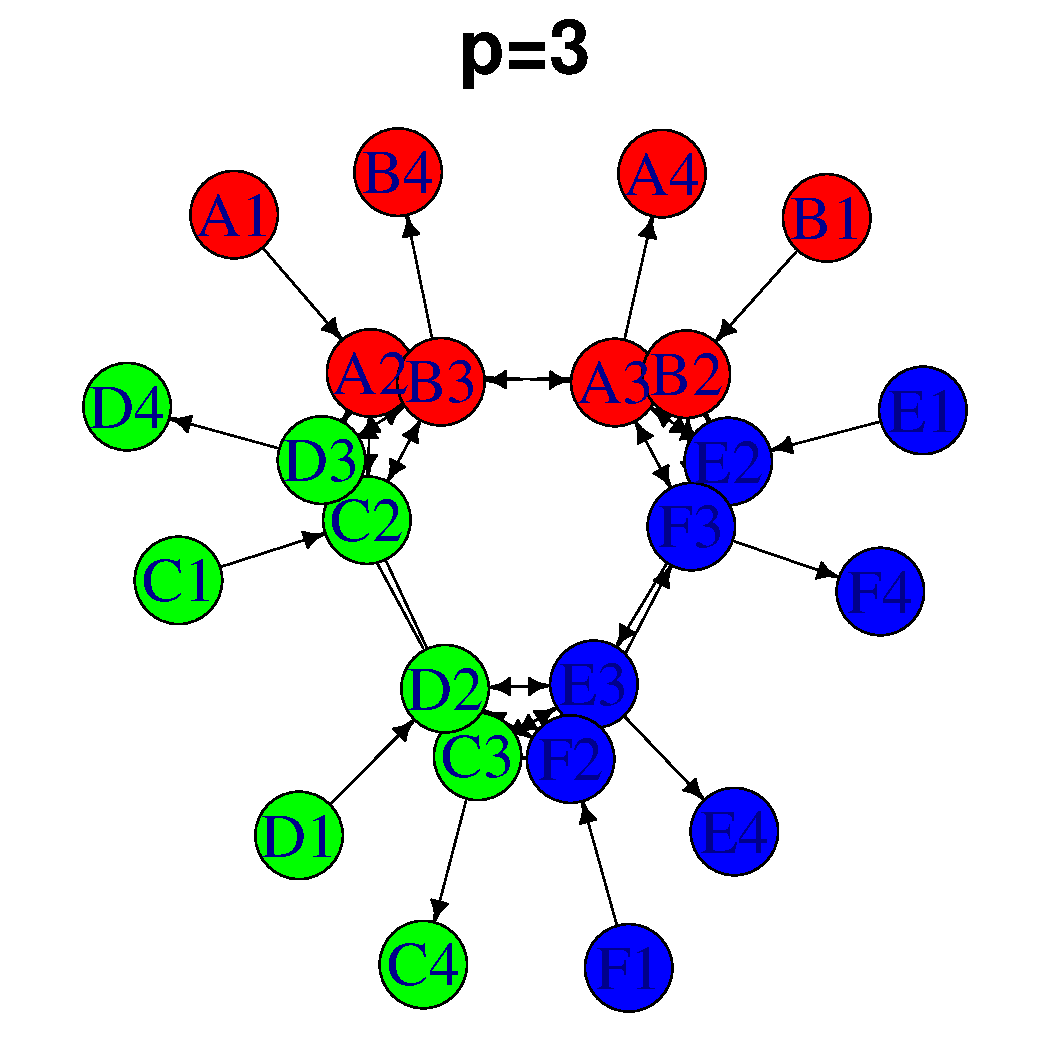
\includegraphics[width=0.3\textwidth]{fig/toy_3_display.pdf}
	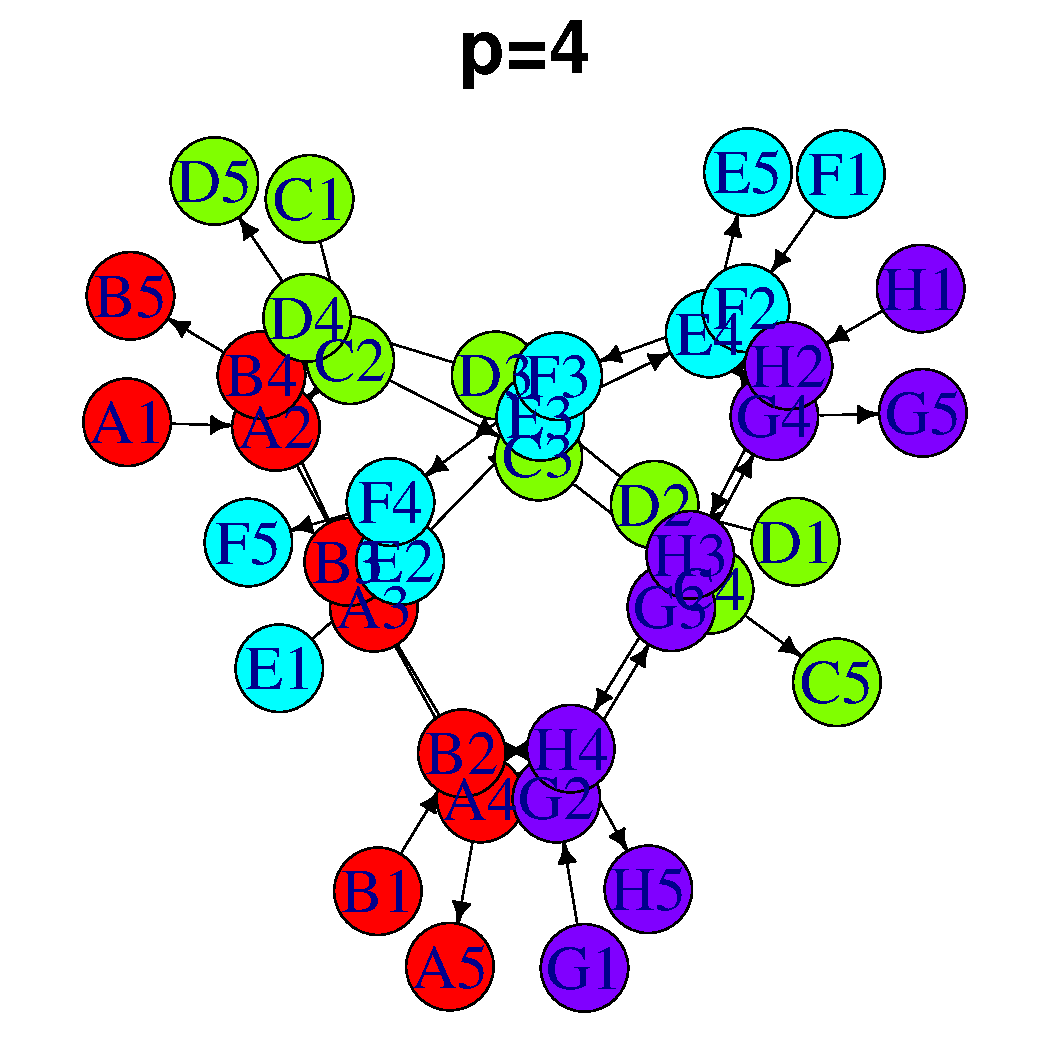
\includegraphics[width=0.3\textwidth]{fig/toy_4_display.pdf}
	\caption{3 toy examples, with the number of tours $p \in \{2,3,4\}$. Tours are displayed in the same color, line have a unique letter, and each stop a unique combination of a letter and a number. Clusters of nodes represent positions where transfer between tours are possible.}
	\label{toy_example_plots}
\end{figure}

Allowed origin-destination pairs $(s,t)$ are constructed with the same set of rules found in (REF), but without considering the exclusion criterion based on the pedestrian distance, as nodes are not spatially located. The graph shortest-path structure for the allowed origin-destination pairs is stored in the edge-trip incidence matrix $\bm{\chi}$.

A transportation flow $\mathbf{N}_\text{ref} = (n^\text{ref}_{st})$ is drawn by setting a fixed number of passengers $n^\text{ref}_{\bullet \bullet}$, and each passenger is assigned randomly to a $(s, t)$ pair drawn uniformly among all allowed origin-destination pairs. From this reference transportation flow $\mathbf{N}_\text{ref}$, using the edge-trip incidence matrix $\bm{\chi}$ and equation (\ref{equationGG}), we can compute flow on edges $\mathbf{X}_\text{ref}$ and, in turn, the number of passengers embarking $\mathbf{a}_\text{ref}$ and the number of passengers disembarking $\mathbf{b}_\text{ref}$ at each stop.

\subsubsection{Error measurements}
\label{error_measures}
Using the network structure, $\mathbf{a}_\text{ref}$, $\mathbf{b}_\text{ref}$, we can obtain a estimation of the real flow through the algorithm, noted $\mathbf{N} = (n_{st})$. There are two types of dissimilarity measure between the real data and the solution proposed by the algorithm: (1) how much $\mathbf{N}$ differs from $\mathbf{N}_\text{ref}$, and (2) how well constraints defined by the number of passengers embarking $\mathbf{a}_\text{ref}$ and disembarking $\mathbf{b}_\text{ref}$ are respected. The first dissimilarity is measured through the \emph{mean transportation error}, denoted by $\text{MTE}(\mathbf{N})$, and computed with
\begin{equation}
	\text{MTE}(\mathbf{N}) = \sum_{st} \frac{n^\text{ref}_{st}}{n^\text{ref}_{\bullet \bullet}} \frac{\lvert n_{st} - n^\text{ref}_{st}\lvert}{n^\text{ref}_{st}} = \frac{\sum_{st} \lvert n_{st} - n^\text{ref}_{st}\lvert}{n^\text{ref}_{\bullet \bullet}} 
	\label{MTE}
\end{equation} 
and the second one with the \emph{mean margin error}, noted $\text{MME}(\mathbf{N})$, obtained with
\begin{align}
	\text{MME}(\mathbf{N}) &= \frac{1}{2} \sum_{i} \frac{a^\text{ref}_i}{a^\text{ref}_\bullet} \frac{\lvert z_{\bullet i} + n_{i \bullet} - a^\text{ref}_i \lvert}{a^\text{ref}_i} + \frac{1}{2} \sum_{i} \frac{b^\text{ref}_i}{b^\text{ref}_\bullet} \frac{\lvert z_{i \bullet} + n_{\bullet i} - b^\text{ref}_i \lvert}{a^\text{ref}_i} \notag \\
	&= \frac{\sum_i (\lvert z_{\bullet i} + n_{i \bullet} - a^\text{ref}_i \lvert + \lvert z_{i \bullet} + n_{\bullet i} - b^\text{ref}_i \lvert)}{2n^\text{ref}_{\bullet \bullet}}
	\label{MME}
\end{align} 
where $z_{ij} = I((i,j) \in \mathcal{T})\sum_{st} \chi_{ij}^{st} n_{st}$ is the flow on transfer edges $\mathcal{T}$. 

Note that, by construction, the mean margin error should be null when the algorithm converge. However, it can be informative to track down this error along iterations and, in some practical cases where the network is large, the algorithm convergence criterion is reached without having margin constraints perfectly respected.


\subsubsection{Algorithm iterations}
\label{example_construction}

\begin{figure}
	\label{iteration_plots}
	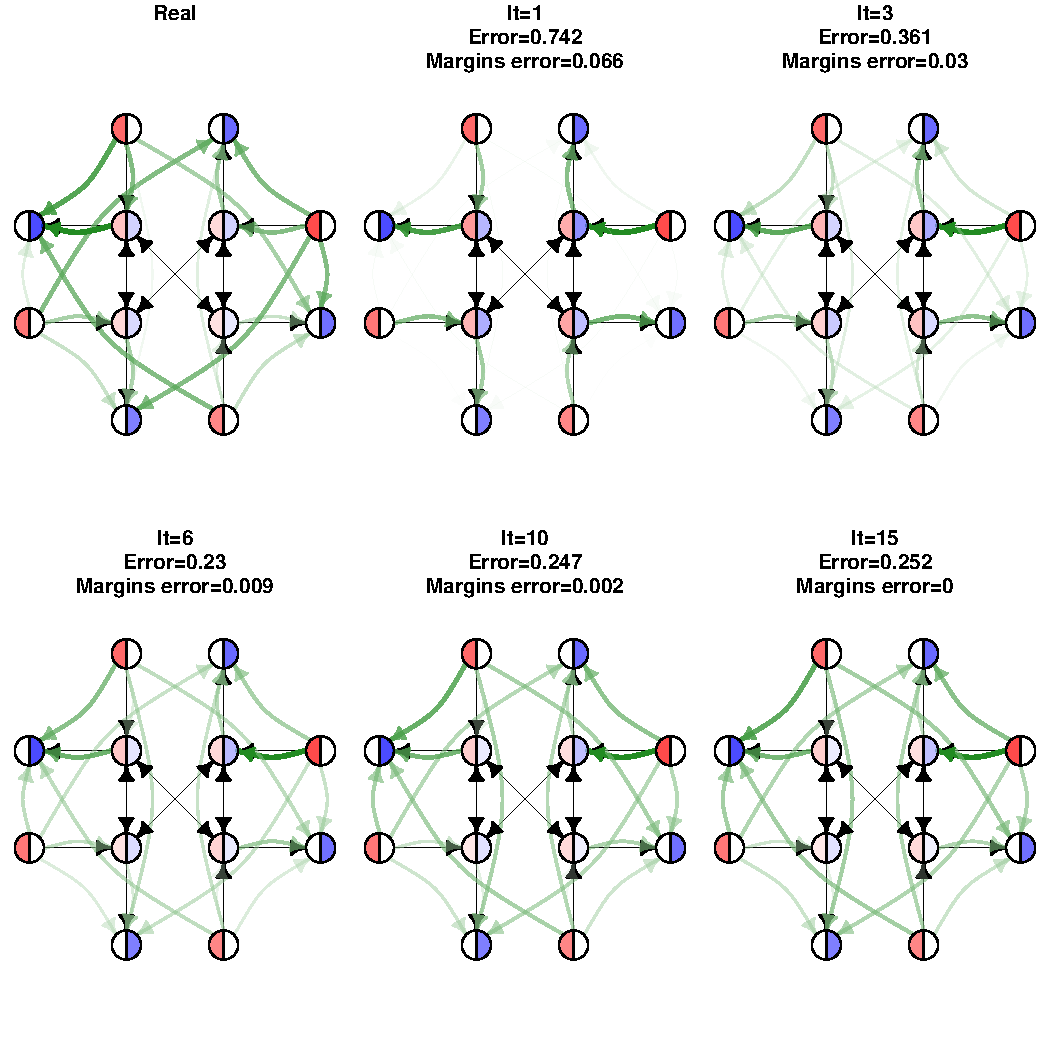
\includegraphics[width=0.98\textwidth]{fig/iterations.pdf}
	\caption{Blabla}
\end{figure}


\subsection{Real Data}

%% --------------------------------- CONCLUSION

\section{Conclusion}

  
\newpage


\section*{Appendix}
Text for this section\ldots

%%%%%%%%%%%%%%%%%%%%%%%%%%%%%%%%%%%%%%%%%%%%%%
%%                                          %%
%% Backmatter begins here                   %%
%%                                          %%
%%%%%%%%%%%%%%%%%%%%%%%%%%%%%%%%%%%%%%%%%%%%%%

\begin{backmatter}

\section*{Acknowledgements}%% if any
Text for this section\ldots

\section*{Funding}%% if any
Text for this section\ldots

\section*{Abbreviations}%% if any
Text for this section\ldots

\section*{Availability of data and materials}%% if any
Text for this section\ldots

\section*{Ethics approval and consent to participate}%% if any
Text for this section\ldots

\section*{Competing interests}
The authors declare that they have no competing interests.

\section*{Consent for publication}%% if any
Text for this section\ldots

\section*{Authors' contributions}
Text for this section \ldots

\section*{Authors' information}%% if any
Text for this section\ldots

%%%%%%%%%%%%%%%%%%%%%%%%%%%%%%%%%%%%%%%%%%%%%%%%%%%%%%%%%%%%%
%%                  The Bibliography                       %%
%%                                                         %%
%%  Bmc_mathpys.bst  will be used to                       %%
%%  create a .BBL file for submission.                     %%
%%  After submission of the .TEX file,                     %%
%%  you will be prompted to submit your .BBL file.         %%
%%                                                         %%
%%                                                         %%
%%  Note that the displayed Bibliography will not          %%
%%  necessarily be rendered by Latex exactly as specified  %%
%%  in the online Instructions for Authors.                %%
%%                                                         %%
%%%%%%%%%%%%%%%%%%%%%%%%%%%%%%%%%%%%%%%%%%%%%%%%%%%%%%%%%%%%%

% if your bibliography is in bibtex format, use those commands:
\bibliographystyle{bmc-mathphys} % Style BST file (bmc-mathphys, vancouver, spbasic).
\bibliography{article_tl.bib}      % Bibliography file (usually '*.bib' )
% for author-year bibliography (bmc-mathphys or spbasic)
% a) write to bib file (bmc-mathphys only)
% @settings{label, options="nameyear"}
% b) uncomment next line
%\nocite{label}

% or include bibliography directly:
% \begin{thebibliography}
% \bibitem{b1}
% \end{thebibliography}

%%%%%%%%%%%%%%%%%%%%%%%%%%%%%%%%%%%
%%                               %%
%% Figures                       %%
%%                               %%
%% NB: this is for captions and  %%
%% Titles. All graphics must be  %%
%% submitted separately and NOT  %%
%% included in the Tex document  %%
%%                               %%
%%%%%%%%%%%%%%%%%%%%%%%%%%%%%%%%%%%

%%
%% Do not use \listoffigures as most will included as separate files

\section*{Figures}
  \begin{figure}[h!]
  \caption{Sample figure title}
\end{figure}

\begin{figure}[h!]
  \caption{Sample figure title}
\end{figure}

%%%%%%%%%%%%%%%%%%%%%%%%%%%%%%%%%%%
%%                               %%
%% Tables                        %%
%%                               %%
%%%%%%%%%%%%%%%%%%%%%%%%%%%%%%%%%%%

%% Use of \listoftables is discouraged.
%%
\section*{Tables}
\begin{table}[h!]
\caption{Sample table title. This is where the description of the table should go}
  \begin{tabular}{cccc}
    \hline
    & B1  &B2   & B3\\ \hline
    A1 & 0.1 & 0.2 & 0.3\\
    A2 & ... & ..  & .\\
    A3 & ..  & .   & .\\ \hline
  \end{tabular}
\end{table}

%%%%%%%%%%%%%%%%%%%%%%%%%%%%%%%%%%%
%%                               %%
%% Additional Files              %%
%%                               %%
%%%%%%%%%%%%%%%%%%%%%%%%%%%%%%%%%%%

\section*{Additional Files}
  \subsection*{Additional file 1 --- Sample additional file title}
    Additional file descriptions text (including details of how to
    view the file, if it is in a non-standard format or the file extension).  This might
    refer to a multi-page table or a figure.

  \subsection*{Additional file 2 --- Sample additional file title}
    Additional file descriptions text.




\end{backmatter}
\end{document}
